\documentclass[12pt]{beamer}
\title{Improvements in LARFT inside LAPACK}
\author{Johnathan Rhyne\\Advised by: Julien Langou}
\institute{University of Colorado Denver}
\usepackage{algorithm}
\usepackage{algpseudocode}
\date{\today}

\begin{document}
    \begin{frame}
        \titlepage
    \end{frame}
    % Table of contents. Can be helpful for navigating after the fact
    \begin{frame}
        \frametitle{Overview}
        \tableofcontents
    \end{frame}
    \section{Preliminaries}
    \begin{frame}
        %
        %LAPACK stands for Linear Algebra PACKage, which provides a suite of routines to 
        %perform many linear algebra operations including but not limited to:
        %
        \frametitle{What is LAPACK}
        LAPACK provides interfaces for:
        \begin{enumerate}
            \item Matrix multiplication
            \item Solving linear systems of equations
            \item Factorizing matrices
        \end{enumerate}
        and more!
        %
        %We provide the interface and then set a baseline for chip vendors like INTEL and AMD to either package
        %or beat themselves.
        %
    \end{frame}
    \begin{frame}
        \frametitle{Brief Linear Algebra Review}
        Householder reflectors are a way to to represent a matrix as a product of rank $1$ updates of the form
        $$
            \left(I - \tau_1 v_1v_1^\top\right)\cdots\left(I - \tau_k v_kv_k^\top\right) = VTV^\top
        $$
        Routines that use this\footnote{Collected by listing some functions found on the caller graph of DLARFT found \textcolor{blue}{\href{https://netlib.org/lapack/explore-html//d7/d0d/group__larft_ga20e5a4f351b3ca7d30078547e55884f5_ga20e5a4f351b3ca7d30078547e55884f5_icgraph_org.svg}{here}}}
        \begin{itemize}
            \item SVD *GESVD
            \item Hessenberg Reduction *GEQRF
            \item QR Factorization *ORGQR
        \end{itemize}
    \end{frame}
    \section{Existing Behavior}
    \begin{frame}
        \frametitle{LAPACK Implementation}
        % At a high level, what the current dlarft does is compute T one column at a time.
        The algorithm for DLARFT is given by\footnote{Taken from the comments of DLARFT found \textcolor{blue}{\href{https://netlib.org/lapack/explore-html//dd/daa/dlarft_8f_source.html}{here}}\\\,}:
        \begin{algorithmic}
            \For{Each column of $V$}
                \State $T(:,i) = -\tau_i V(:,1:i-1)^\top * V(:,i)$
                \State $T(:,i) = T(:,1:i-1) * T(:,i)$
                \State $T(i,i) = \tau_i$
            \EndFor
        \end{algorithmic}

        % As we can see above, we are doing a bunch of matrix-vector operations. This leads to two kinds of improvements
        % The first being in restructuring the code to be recursive as this scheme can lead to performance gains
        % particularly when we have many more rows than columns
    \end{frame}
    \section{New Behavior}
    \subsection{Recursive LARFT}
    \begin{frame}
        \frametitle{Recursive Implementation}
        % In order to motivate the recursive formulation, we notice that if we had a way to collect these
        % T values for the first l columns and the remaining, we want to do the following
        If we collect only some of the reflectors on the first and second half, we get
        \begin{align*}
            &\,(I - V_1T_1V_1^\top)(I - V_2T_2V_2^\top) \\
            &= I - V_1T_1V_1^\top - V_2T_2V_2^\top + V_1T_1V_1^\top V_2T_2V_2^\top
        \end{align*}
        Can be rewritten as:
        $$
            I - VTV^\top
        $$
        where:
        % Then, if we define T_3 and V as follows, we can recover above!
        \begin{align*}
            T_3 &= -T_1V_1^\top V_2T_2 \\
            V &= \begin{bmatrix}
                V_1 & V_2
            \end{bmatrix}
        \end{align*}
    \end{frame}
    \subsection{Matrix Operation LARFT}
    \begin{frame}
        \frametitle{Matrix Operation Implementation}
        Based on the work done by Joffrain and Low \footnote{Accumulating Householder Transformations, Revisited} and Puglisi \footnote{Modification of the Householder method based on the compact wy representation}
        \\\,\\
        \begin{algorithmic}
            \State $T = V^\top V$ (Only upper triangular part)
            \State Scale the diagonal by $\frac{1}{2}$.
            \State $T = T^{-1}$.
        \end{algorithmic}
        \,\\\,\\
        For more details about why this works, see either Theorem 2 from Joffrain and Low or the algorithm from Puglisi
    \end{frame}
    \section{Numerical Results}
    \begin{frame}
        \frametitle{Numerical Results}
        We ran the following tests on the Alderaan\footnote{Specifications for the cluster can be found \textcolor{blue}{\href{https://ccm-docs.readthedocs.io/en/latest/alderaan\#hardware}{here}}\\\,} cluster here at UC Denver\\
        % put pictures here of just the times.
        \begin{center}
        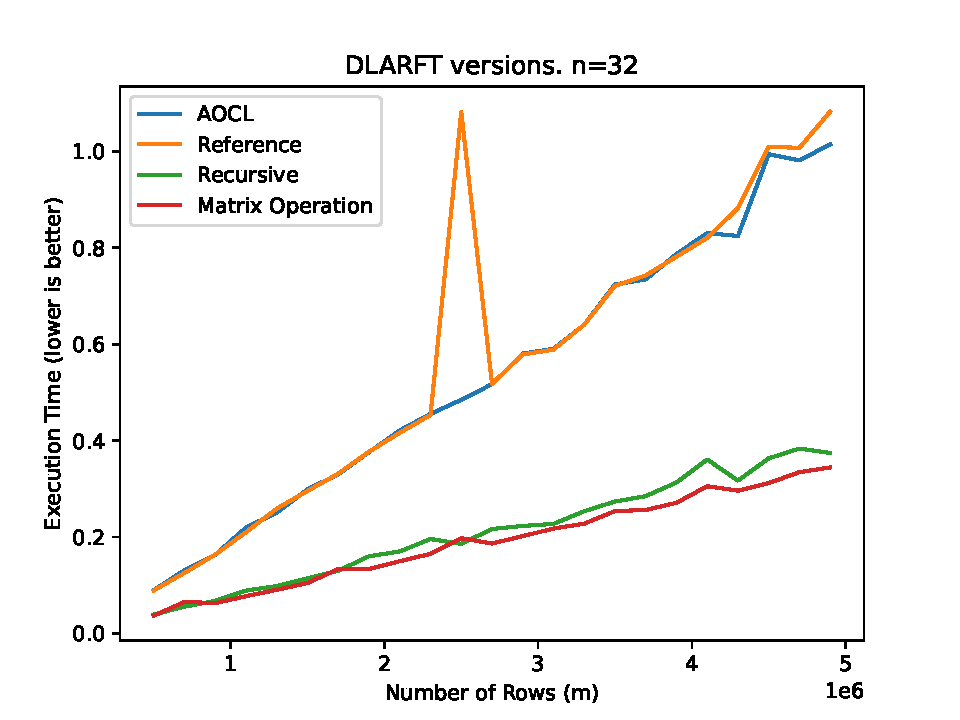
\includegraphics[width=.4\textwidth]{figs/dlarftNBTime.pdf}
        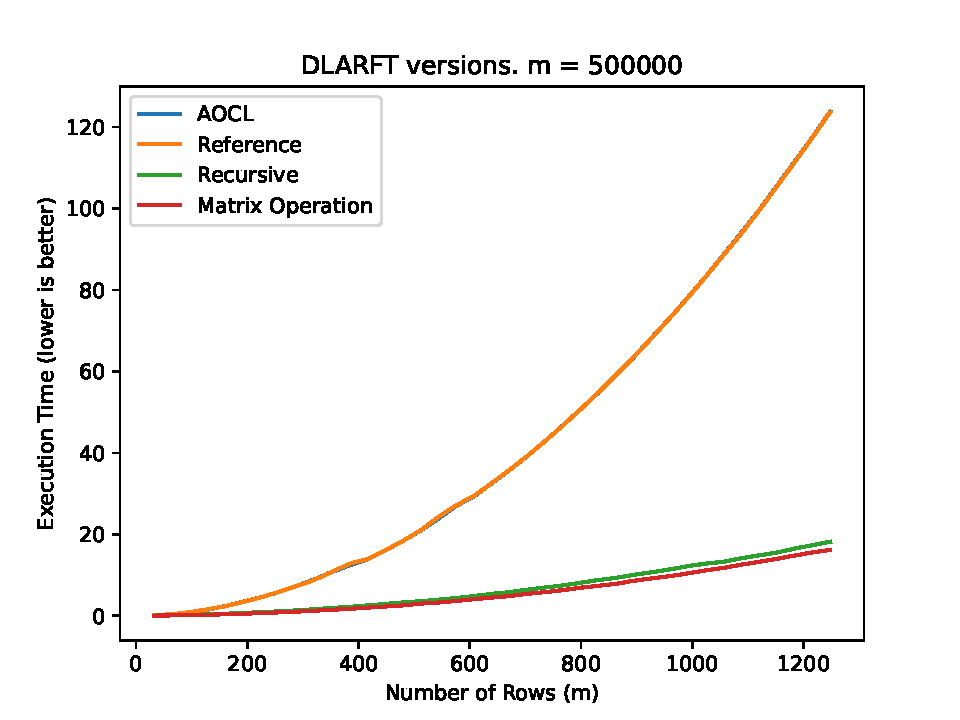
\includegraphics[width=.4\textwidth]{figs/dlarftNVaryTime.pdf}
        \end{center}
    \end{frame}
    \section{Future work}
    \begin{frame}
        \frametitle{Future work/open questions for Matrix Operation Based}
        \begin{itemize}
            \item Complex arithmetic
            \item Stability
        \end{itemize}
    \end{frame}
    % Dummy frame used for ease of copy and pasting
    % Complex?
    %\begin{frame}
    %    \frametitle{a}
    %\end{frame}
\end{document}
